\subsection{Procedure}

Thus far, the problem has been introduced and the required terminologt has been defined. Recall that there are two 
changes; the insertion/deletion of bars or repositioning bars.
However, there has yet to be discussion regarding the two 
listing algorithms. In the procedure section 
we look at each of the algorithms and explain what 
each of the algorithms are doing. The goal is to transition from 
$L_{i}$ to $L_{i+1}$ in $CanL{\pi_{N}}$ with minimal change, which means adding or removing 
the least number of bars to get from $L_{i}$ to $L_{i+1}$ or relocating 
the least number of bars to get from $L_{i}$ to $L_{i+1}$.\par 

The reason that the modified SJT and CI algorithms were chosen is because they allow 
for minimal change from $L_{i}$ to $L_{i+1}$. While conducting this research, modifications 
to the permutation listing algorithms mentioned in chapter one were applied. Recall that 
these listing algorithms were Zaks, Heaps, and Lexicographic. These listing algorithms 
did not allow for minimal change when transitioning from $L_{i}$ to $L_{i+1}$.
%%section SJT
\subsubsection{Steinhaus-Johnson-Trotter}
\begin{algorithm}
  \caption{Modified SJT algorithm for processing at $K=N$}
  \begin{algorithmic}[1]
    \Function{modifiedSjt}{$N$, $Ladder[2(N-1)-1][N-1]$, $Arr[N-1]$, $Direction[N]$}


      \State $print(Ladder)$

      %%base case
      \If{$globalCount = N!$}
        \State return
      \EndIf

     
      \State $dir \gets direction[N]$
      \State $K \gets N-1$
      %%swap the nth element n-1 times
      \For{$i \gets 1$,$i < N$, $i \gets i+1$}
        
        \If{$dir = left$}
            \State $row \gets (N) - i$
            \State $col \gets row$
            \State $ladder[row][col] \gets 1$
        \Else
            \State $row \gets i$
            \State $col \gets row$
            \State $ladder[row][col] \gets 0$
        \EndIf
        \State $globalCount \gets globalCount+1$
        \State $print(Ladder)$

      \EndFor
      \State $direction[N] \gets !direction[N]$
      \State $HELPERSJT(K, N, ladder, arr, direction)$
      \State $MODIFIEDSJT(N,  ladder, arr, direction)$

    \EndFunction
  \end{algorithmic}
\end{algorithm}

%%helper algorithm
\begin{algorithm}
  \caption{Helper SJT algorithm for processing when $2 \leq K < N$}
  \begin{algorithmic}[1]
    \Function{helpersjt}{$N$, $K=(N-1)$, $Ladder[2(N-1)-1][N-1]$, $Arr[N-1]$, $Direction[N]$}

      \For{$i \gets K$, $i \geq 1$, $i \gets i-1$}
        \If{$arr[K] < K$}
        \State $globalCount \gets globalCount + 1$

          \If{$dir[K] = LEFT$}
            \State $row \gets (N-1) + (N-K) - arr[K]$
            \State $col \gets (K) - arr[K]$
            \State $ladder[row][col] \gets 1$

          \Else
            \State $row \gets  (N-1) + (N-K) + arr[K] - (K-2)$
            \State $col \gets arr[K]$
            \State $ladder[row][col] \gets 0$
          \EndIf
          \State $arr[K]\gets arr[K]+1$
          \State return
        \Else 
          \State $arr[K] \gets 0$
          \State $direction[K] \gets !direction[K]$
        \EndIf
        $K \gets K-1$
      \EndFor
      \EndFunction
  \end{algorithmic}
\end{algorithm}
\pagebreak

Let the \emph{identity ladder} be the ladder for the sorted permutation from $[1 \dots N]$.
Let the initial conditions of the algorithm be the fallowing. The $Ladder= 2D array$,  
let $n \geq 1$, let $arr$ be set to zero for all indexes. Let $dir$ be set to false 
for all indexes. The principles of the algorithm are the following, if the direction for a 
given route is false, then bars will be added for that given route, from right to left, bottom to top, until no more bars can be added. Let a 
$1$ at $Ladder[row][col]$ indicate a bar has been added to the ladder at the given row and column.
If the direction for a given route is true, then bars will be removed for that given route, left to right, top to bottom, until 
no more bars can be removed. Let a $0$ at $Ladder[row][col]$ indicate a bar has been removed from the ladder 
at the given row and column. Let $K$ be the value of some given route where $1 < K <= N$. Note that element one has no route.
The number of bars for a given route is $1 \leq K < N$. This is because the maximum number of inversions 
the $kth$ element can make is $K-1$, therefore the $kth$ route can have at most $N-1$, if $K=N$, and 
at least $1$ bar if $K=2$. Once all the bars for the $Kth$ route have been added 
or removed, the direction for the $Kth$ route is switched, indicating that its bars will be removed if they 
were added, or added if they were removed. Once all the bars for the $Kth$ route have been added or removed, 
the next bar of the $K-1th$ route will be added or removed. Once this is done, the bars of route $K$ will 
then be added if they were previously removed or removed if previously added. Repeat this process until all
$N!$ ladders have been generated.


%%prove the dimensions of the datastructure
\begin{theorem}
  The number of rows required for the ladder data-structure is $2(N-1) - 1$ and the number of columns required for 
  the ladder is $N-1$.
\end{theorem}
\begin{proof}
  The number of columns is fairly straighforward. Seeing as there are always $N$ elements in $\pi_{N}$, 
  a column represents a gap between lines in the corresponding ladder-lottery. Let $Line_{i}$ be a vertical line in a ladder-lottery 
  with some element in $\pi_{N}$ at the top of the line and the $ith$ element in $\pi_{N}$ be 
  at the bottom of $Line_{i}$. There are $N$ lines in the ladder-lottery, a column in the ladder data-structure
  simply represents a gap between two adjacent lines in the ladder lottery.\par 
  The number of rows for the ladder data-structure is calculated a follows, given $\pi_{N}$, the minimal 
  number of rows required is when $\pi_{N}$ is sorted. In this case there are zero rows because there are 
  zero bars added to the ladder. This ladder is $L_{N_{ID}}$ and is 
  the first ladder in $CanL{\pi_{N}}$. When a bar is added to the ladder it can be added to an already existing row 
  or to a new row. If the current state of the ladder is $L_{N_{ID}}$ then the new bar will create the $N-1$th row in the 
  $N-1$th column. Let the bar belong to the $Nth$ route, then repeat adding bars for the $Nth$ route, bottom to top left to right. 
  Since no two bars of the $Nth$ route can be on the same row, this will require $N-1$ rows. Note, if they were added to the same 
  row, then the left end point of the right bar would be touching the right end point of the left bar which is disallowed. Once the 
  bars of the $Nth$ element are added, the bars of the $N-1th$ route will be added. The $N-1th's$ first bar 
  will be added to the $N-2$ column, otherwise it would be directly below the first bar of the $Nth$ route, which is a violation. 
  Since the first bar of the $N-1$'s element is added to column $N-2$, then it must be given a new row, otherwise its right end point 
  will be touching  the left end point of the first bar of route $N$. The remaining $N-2$ bars of element $N-1$
  will be added bottom right to top left, but none of their end points will touch the end points of element $N$ seeing as they will 
  always be two columns apart from any bar in $N's$ route. The same logic applies to element $N-2$, it will require one extra row for its 
  first bar, in order not to touch the first bar of element $N-1$, but the remainder of its bars will always be two columns away from 
  the remainder of the bars for $N-1$, etc. Therefore there are $N-2$ rows required for each element, $K$,  $2 \leq K < N$. Note that element 
  $1$ has no bars in its route. Therefore there are $(N-1)$ rows required for element $N's$ route plus $(N-2)$ rows required for 
  elements $2 \leq K < N$. In conclusion the number of rows required is $(N-1) + (N-2) = 2(N-1)-1$. See figure for the tree of ladders 
  generated by modified SJT for $N=4$
\end{proof}



\begin{figure}[!htp]
\begin{center}
  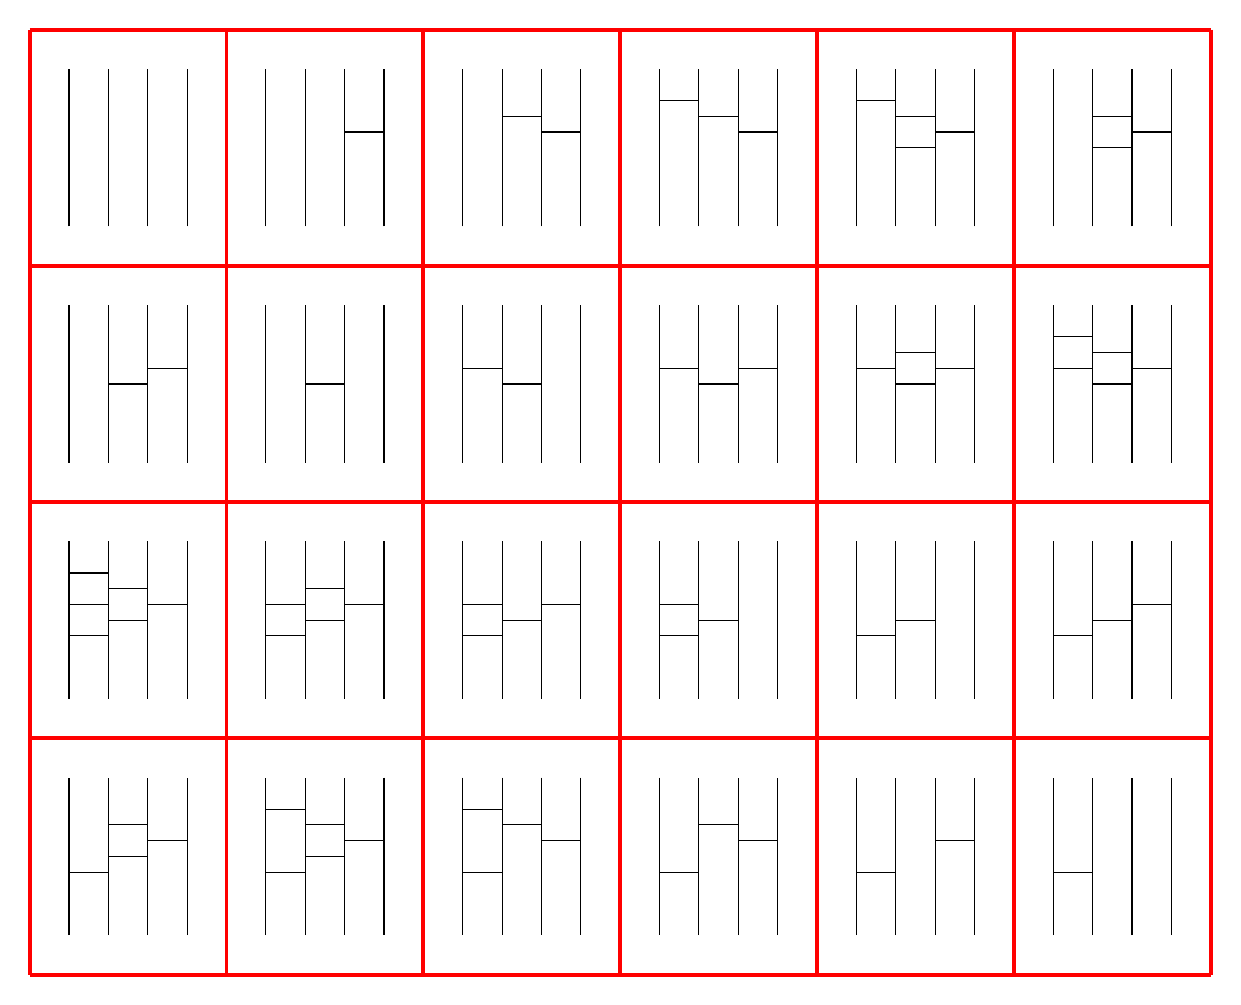
\begin{tikzpicture}
    \draw(0, 0) to (0, 2);
    \draw(0.5, 0) to (0.5, 2);
    \draw(1, 0) to (1, 2);
    \draw(1.5, 0) to (1.5, 2);

    \draw(2.5, 0) to (2.5, 2);
    \draw(3, 0) to (3, 2);
    \draw(3.5, 0) to (3.5, 2);
      \draw(3.5, 1.2) to (4, 1.2);
    \draw(4, 0) to (4, 2);

    \draw(5, 0) to (5, 2);
    \draw(5.5, 0) to (5.5, 2);
      \draw(5.5, 1.4) to (6, 1.4);
    \draw(6, 0) to (6, 2);
      \draw(6, 1.2) to (6.5, 1.2);
    \draw(6.5, 0) to (6.5, 2);

    \draw(7.5, 0) to (7.5, 2);
      \draw(7.5, 1.6) to (8, 1.6);
    \draw(8, 0) to (8, 2);
      \draw(8, 1.4) to (8.5, 1.4);
    \draw(8.5, 0) to (8.5, 2);
      \draw(8.5, 1.2) to (9, 1.2);
    \draw(9, 0) to (9, 2);

    \draw(10, 0) to (10, 2);
      \draw(10, 1.6) to (10.5, 1.6);
    \draw(10.5, 0) to (10.5, 2);
      \draw(10.5, 1.4) to (11, 1.4);
      \draw(10.5, 1) to (11, 1);
    \draw(11, 0) to (11, 2);
      \draw(11, 1.2) to (11.5, 1.2);
    \draw(11.5, 0) to (11.5, 2);

    \draw(12.5, 0) to (12.5, 2);
    \draw(13, 0) to (13, 2);
      \draw(13, 1.4) to (13.5, 1.4);
      \draw(13, 1) to (13.5, 1);
    \draw(13.5, 0) to (13.5, 2);
      \draw(13.5, 1.2) to (14, 1.2);
    \draw(14, 0) to (14, 2);

    %%End of first row
    %%Second row

    \draw(0, -3) to (0, -1);
    \draw(0.5, -3) to (0.5, -1);
      \draw(0.5, -2) to (1, -2);
    \draw(1, -3) to (1, -1);
      \draw(1, -1.8) to (1.5, -1.8);
    \draw(1.5, -3) to (1.5, -1);

    \draw(2.5, -3) to (2.5, -1);
    \draw(3, -3) to (3, -1);
      \draw(3, -2) to (3.5, -2);
    \draw(3.5, -3) to (3.5, -1);
    \draw(4, -3) to (4, -1);

    \draw(5, -3) to (5, -1);
      \draw(5, -1.8) to (5.5, -1.8);
    \draw(5.5, -3) to (5.5, -1);
      \draw(5.5, -2) to (6, -2);
    \draw(6, -3) to (6, -1);
    \draw(6.5, -3) to (6.5, -1);

    \draw(7.5, -3) to (7.5, -1);
      \draw(7.5, -1.8) to (8, -1.8);
    \draw(8, -3) to (8, -1);
      \draw(8, -2) to (8.5, -2);
    \draw(8.5, -3) to (8.5, -1);
      \draw(8.5, -1.8) to (9, -1.8);
    \draw(9, -3) to (9, -1);

    \draw(10, -3) to (10, -1);
      \draw(10, -1.8) to (10.5, -1.8);
    \draw(10.5, -3) to (10.5, -1);
      \draw(10.5, -1.6) to (11, -1.6);
      \draw(10.5, -2) to (11, -2); 
    \draw(11, -3) to (11, -1);
      \draw(11, -1.8) to (11.5, -1.8);
    \draw(11.5, -3) to (11.5, -1);

    \draw(12.5, -3) to (12.5, -1);
      \draw(12.5, -1.4) to (13, -1.4);
      \draw(12.5, -1.8) to (13, -1.8);
    \draw(13, -3) to (13, -1);
      \draw(13, -1.6) to (13.5, -1.6);
      \draw(13, -2) to (13.5, -2);
    \draw(13.5, -3) to (13.5, -1);
      \draw(13.5, -1.8) to (14, -1.8);
    \draw(14, -3) to (14, -1);
    %%End of second row
    \draw(0, -6) to (0, -4);
      \draw(0, -5.2) to (0.5, -5.2);
      \draw(0, -4.4) to (0.5, -4.4);
      \draw(0, -4.8) to (0.5, -4.8);
    \draw(0.5, -6) to (0.5, -4);
      \draw(0.5, -4.6) to (1, -4.6);
      \draw(0.5, -5) to (1, -5);
    \draw(1, -6) to (1, -4);
      \draw(1, -4.8) to (1.5, -4.8);
    \draw(1.5, -6) to (1.5, -4);

    \draw(2.5, -6) to (2.5, -4);
      \draw(2.5, -5.2) to (3, -5.2);
      \draw(2.5, -4.8) to (3, -4.8);
    \draw(3, -6) to (3, -4);
      \draw(3, -4.6) to (3.5, -4.6);
      \draw(3, -5) to (3.5, -5);
    \draw(3.5, -6) to (3.5, -4);
      \draw(3.5, -4.8) to (4, -4.8);
    \draw(4, -6) to (4, -4);

    \draw(5, -6) to (5, -4);
      \draw(5, -5.2) to (5.5, -5.2);
      \draw(5, -4.8) to (5.5, -4.8);
    \draw(5.5, -6) to (5.5, -4);
      \draw(5.5, -5) to (6, -5);
    \draw(6, -6) to (6, -4);
      \draw(6, -4.8) to (6.5, -4.8);
    \draw(6.5, -6) to (6.5, -4);

    \draw(7.5, -6) to (7.5, -4);
      \draw(7.5, -5.2) to (8, -5.2);
      \draw(7.5, -4.8) to (8, -4.8);
    \draw(8, -6) to (8, -4);
       \draw(8, -5) to (8.5, -5);
    \draw(8.5, -6) to (8.5, -4);
    \draw(9, -6) to (9, -4);

    \draw(10, -6) to (10, -4);
          \draw(10, -5.2) to (10.5, -5.2);
    \draw(10.5, -6) to (10.5, -4);
           \draw(10.5, -5) to (11, -5);
    \draw(11, -6) to (11, -4);
    \draw(11.5, -6) to (11.5, -4);

    \draw(12.5, -6) to (12.5, -4);
              \draw(12.5, -5.2) to (13, -5.2);

    \draw(13, -6) to (13, -4);
               \draw(13, -5) to (13.5, -5);

    \draw(13.5, -6) to (13.5, -4);
               \draw(13.5, -4.8) to (14, -4.8);

    \draw(14, -6) to (14, -4);

    %%End of third row

    \draw(0, -9) to (0, -7);
      \draw(0, -8.2) to (0.5, -8.2);
    \draw(0.5, -9) to (0.5, -7);
      \draw(0.5, -8) to (1, -8);
      \draw(0.5, -7.6) to (1, -7.6);
    \draw(1, -9) to (1, -7);
      \draw(1, -7.8) to (1.5, -7.8);
    \draw(1.5, -9) to (1.5, -7);

    \draw(2.5, -9) to (2.5, -7);
      \draw(2.5, -7.4) to (3, -7.4);
      \draw(2.5, -8.2) to (3, -8.2);
    \draw(3, -9) to (3, -7);
      \draw(3, -8) to (3.5, -8);
      \draw(3, -7.6) to (3.5, -7.6);
    \draw(3.5, -9) to (3.5, -7);
       \draw(3.5, -7.8) to (4, -7.8);
    \draw(4, -7) to (4, -9);

    \draw(5, -7) to (5, -9);
      \draw(5, -7.4) to (5.5, -7.4);
      \draw(5, -8.2) to (5.5, -8.2);
    \draw(5.5, -7) to (5.5, -9);
      \draw(5.5, -7.6) to (6, -7.6);
    \draw(6, -7) to (6, -9);
           \draw(6, -7.8) to (6.5, -7.8);
    \draw(6.5, -7) to (6.5, -9);

    \draw(7.5, -7) to (7.5, -9);
          \draw(7.5, -8.2) to (8, -8.2);
    \draw(8, -9) to (8, -7);
        \draw(8, -7.6) to (8.5, -7.6);
    \draw(8.5, -9) to (8.5, -7);
               \draw(8.5, -7.8) to (9, -7.8);
    \draw(9, -9) to (9, -7);

    \draw(10, -9) to (10, -7);
      \draw(10, -8.2) to (10.5, -8.2);
    \draw(10.5, -9) to (10.5, -7);
    \draw(11, -9) to (11, -7);
      \draw(11, -7.8) to (11.5, -7.8);
    \draw(11.5, -9) to (11.5, -7);

    \draw(12.5, -9) to (12.5, -7);
              \draw(12.5, -8.2) to (13, -8.2);
    \draw(13, -9) to (13, -7);
    \draw(13.5, -9) to (13.5, -7);
    \draw(14, -9) to (14, -7);

    %%end fourth row

    %%draw the border

    \draw [line width=0.5mm, red ] (-0.5,2.5) to (-0.5,-9.5);
    \draw [line width=0.5mm, red ] (2,2.5) to (2,-9.5);
    \draw [line width=0.5mm, red ] (4.5,2.5) to (4.5,-9.5);
    \draw [line width=0.5mm, red ] (7,2.5) to (7,-9.5);
    \draw [line width=0.5mm, red ] (9.5,2.5) to (9.5,-9.5);
    \draw [line width=0.5mm, red ] (12,2.5) to (12,-9.5);
    \draw [line width=0.5mm, red ] (14.5,2.5) to (14.5,-9.5);

   \draw [line width=0.5mm, red ] (-0.5,2.5) to (14.5,2.5);
   \draw [line width=0.5mm, red ] (-0.5,-0.5) to (14.5,-0.5);
      \draw [line width=0.5mm, red ] (-0.5,-3.5) to (14.5,-3.5);
   \draw [line width=0.5mm, red ] (-0.5,-6.5) to (14.5,-6.5);
   \draw [line width=0.5mm, red ] (-0.5,-9.5) to (14.5,-9.5);





  \end{tikzpicture}
  \end{center}
  \caption{The table of $CanL{\pi_{4}}$ generated using the modified SJT algorithm. The table is to be read from top left to bottom right. Note that each ladder is the root ladder from each corresponding $OptL{\pi_{4}}$}
\end{figure}

%%end proof


From the above figure, it should be clear that the canonical representative from $CanL{\pi_{N}}$ when using the 
modified SJT algorithm is the root ladder from each $OptL{\pi_{N}}$. Recall that the root ladder is the 
ladder whose bars of a lesser route have not crossed the bars of a greater route. In the case of the 
modified sjt algorithm, transitioning from $L_{i}$ to $L_{i+1}$ involves simply inserting a new bar 
or removing a bar for a given route. Let $K$ be the current route. If a new bar being added belongs to 
route $K$, then the addition of the bar does not violate the property of the root ladder. If the new bar to
be added belongs to route $K-1$, then the bar is added below $K's$ bars, still not violating the property of 
the root ladder. When a bar is removed, that implies it has already been added. Let $L_{i}$ be a 
ladder whose bar is about to be removed, thus transitioning to $L_{i+1}$. Let $L_{i}$ be a root ladder
, then removing a bar from $L_{i}$ cannot make $L_{i+1}$ a non-root ladder, because 
removing a bar from $L_{i}$ does not allow the bar of a lesser element to cross the bars of a greater element.
Thus, the canonical representative for $CanL{\pi_{N}}$ is always the root ladder from each $OptL{\pi_{N}}$.\par 



%%Beging the cases
The calculations for the row and column for the bar 
depend on several factors. The first factor is whether the row and column is being calculated for $K=N$ or 
if $K < N$. If $K=N$, then the row and column are calculated using the main function, modifiedSJT. The second factor 
is whether a bar is being removed from the ladder or a bar is being added to the ladder. Therefore, there are eight cases 
to consider. The cases are the following: 
\begin{caseof}
  \case{$Route = N$}{Bar is being added. Row is being calculated.}
  \case{$Route = N$}{Bar is being added. Column is being calculated.}
  \case{$Route = N$}{Bar is being removed. Row is being calculated.}
  \case{$Route = N$}{Bar is being removed. Column is being calculated.}
  \case{$Route < N$}{Bar is being added. Row is being calculated.}
  \case{$Route < N$}{Bar is being added. Column is being calculated.}
  \case{$Route < N$}{Bar is being removed. Row is being calculated.}
  \case{$Route < N$}{Bar is being removed. Column is being calculated.}
\end{caseof}

%%End the cases

When proving the above cases, keep in mind that the ladder, $L$, is a two dimensional array with $2(N-1)-1$ rows and $(N-1)$ columns.

%%proof 1
\begin{lemma}
  Let $route=N$. Let $I=$ the current number of bars in the ladder belonging to route $N$. 
  Assume a bar is being added. Then the $row=(N-1)-I$.
\end{lemma}
\begin{proof}
  Keeping in mind we are only dealing with root ladders, then the bars of the $Nth$ route will be above the bars of 
  any other route. The bars are added bottom right to top left, and no two bars of the $Nth$ route can be on the same row, 
  for having two bars of the same route on the same row violates the constraint that no two endpoints of two bars can be toucing.
  There are a total of $N-1$ rows requried for the bars of the $Nth$ route. $I$ is incremented for each bar that is added 
  to the $Nth$ route. The first bar to be added will be at row $N-1$, once it is added $I$ is incremented by one, the second 
  bar of the $Nth$ route will be added to row $N-2$, which equals $N-1-I$. Then $I$ is incremented again. This continues 
  until all bars of the $Nth$ route are added. Refer to figure --fig for an example of row calulation when adding a bar 
  for the $Nth$ route.
\end{proof}\pagebreak


\begin{figure}[!htp]
  \begin{center}
    \begin{tikzpicture}
      \draw(0, 0) to (0, 6);
      \draw(2, 0) to (2, 6);
        \node at(3, 4.7){4,2};
        \draw(2, 4.5) to (4, 4.5);
      \draw(4, 0) to (4, 6);
        \node at(5, 3.7){4,3};
        \draw(4, 3.5) to (6, 3.5);
      \draw(6, 0) to (6, 6);

      \node at(-2, 5.5){R1};
      \node at(-2, 4.5){R2};
      \node at(-2, 3.5){R3};
      \node at(-2, 2.5){R4};
      \node at(-2, 1.5){R5};

      \node at(0, 6.2){1};
      \node at(2, 6.2){4};
      \node at(4, 6.2){2};
      \node at(6, 6.2){3};

      \draw (1,5.5) ellipse (1cm and .4cm);

    \end{tikzpicture}
  \end{center}
  \caption{The row of the last bar to be added for element $4$ is row $1$. $row=1=3-2=(N-1)-I$}
\end{figure}

%%end proof 1


%%Prove case 2
\begin{lemma}
  Let $route=N$. Let $I=$ the current number of bars in the ladder belonging to route $N$. 
  Assume a bar is being added. Then the $column=(N-1)-I$.
\end{lemma}
\begin{proof}
  Keeping in mind we are only dealing with root ladders, then the bars of the $Nth$ route will be above the bars of 
  any other route. The bars are added bottom right to top left. The ladder has a total of $N-1$ columns, seeing as 
  the $Nth$ element has $N-1$ bars, each requiring their own column. If two bars of the $Nth$ element were 
  in the same column, then this would violate one of two constraints. Either the two bars would be directly 
  above/below each other, in which case the ladder would not be optimal seeing as the two elements that crossed the 
  top bar would then cross the bottom bar, which means the ladder has an extra bar. The second case can be discredited as 
  follows. Let the top bar belonging to route $N$ be designated as $X$, let the bottom bar belonging to route $N$ be 
  designated as $Y$. Assume $X$ and $Y$ are in the same column.
  Then there is some third bar $Z$, not belonging to route $N$ and not in the same column 
  as $X$ and $Y$ such that $Z$ is in the column directly to the left or right of the column of $X$ and $Y$. But if that 
  is the case, then $Z$ is above bar $Y$ which violates the definition of the root ladder. Therefore, every bar 
  belonging to route $N$ requires its own column. The first bar to be added to route $N$ goes in the rightmost column which 
  equals column $N-1$, then $I$ is incremented by one. The second bar is in columb $(N-1)-1=(N-1)-I$ and $I$ is incremented 
  by one. The process continues until all $(N-1)$ bars of the $Nth$ route have been added. See figure --fig for an example 
  of column calculation.
\end{proof}

\begin{figure}[!htp]
  \begin{center}
    \begin{tikzpicture}
       \draw(0, 0) to (0, 6);
      \draw(2, 0) to (2, 6);
        \node at(3, 4.7){4,2};
        \draw(2, 4.5) to (4, 4.5);
      \draw(4, 0) to (4, 6);
        \node at(5, 3.7){4,3};
        \draw(4, 3.5) to (6, 3.5);
      \draw(6, 0) to (6, 6);

      \node at(1, -0.3){Col 1};
      \node at(3, -0.3){Col 2};
      \node at(5, -0.3){Col 3};

      \node at(0, 6.2){1};
      \node at(2, 6.2){4};
      \node at(4, 6.2){2};
      \node at(6, 6.2){3};

      \draw (1,5.5) ellipse (1cm and .4cm);


      
    \end{tikzpicture}
  \end{center}
  \caption{The column of the last bar to be added for element $4$ is $1$. $column=1=3-2=(N-1)-I$}
\end{figure}
%%End proof of case 2


%%Proof of case 3
\begin{lemma}
  Let $route=N$. Let $I=$ the current number of bars that have been removed from route $N$. Assume a bar is being removed. 
  Then the $row=I+1$
\end{lemma}
\begin{proof}
  Keeping in mind we are dealing with root ladders and bars are removed from left to right, top to bottom, then the first bar to 
  be removed from route $N$ is at row one. Since no bars have been removed, $I$ currently equals zero, 
  thus row $1=I+1$. Once removed, $I$ is increased by one, indicating a bar has been removed. The next bar is at row two, 
  which again equals $I+1$. Continue until all bars of the $Nth$ route have been removed. See figure --fig for an example 
  of row calculation when removing a bar for the $Nth$ element.
\end{proof}
\begin{figure}[!htp]
  \begin{center}
    \begin{tikzpicture}
      \draw(0, 0) to (0, 6);
        \draw [dashed] (0,5.5) -- (2,5.5);
      \draw(2, 0) to (2, 6);
        \node at(3, 4.7){4,2};
        \draw(2, 4.5) to (4, 4.5);
      \draw(4, 0) to (4, 6);
        \node at(5, 3.7){4,3};
        \draw(4, 3.5) to (6, 3.5);
      \draw(6, 0) to (6, 6);

      \node at(-2, 5.5){R1};
      \node at(-2, 4.5){R2};
      \node at(-2, 3.5){R3};
      \node at(-2, 2.5){R4};
      \node at(-2, 1.5){R5};

      \node at(0, 6.2){1};
      \node at(2, 6.2){4};
      \node at(4, 6.2){2};
      \node at(6, 6.2){3};

      \draw (3,4.5) ellipse (1cm and .4cm);

    \end{tikzpicture}
  \end{center}
  \caption{The row of the second bar to be removed from element $4's$ route is row $2$. The dashed bar indicates that it has already been 
  removed from $4's$ route. $I$ is the number of bars currently removed from $4's$ route, which is currently $1$. Therefore $row=2=I+1$}
\end{figure}

%%End of proof of case 3


%%Proof Case 4
\begin{lemma}
  Let $route=N$. Let $I=$ the current number of bars that have been removed from route $N$. Assume a bar is being removed.
  Then the $column=I+1$.
\end{lemma}
\begin{proof}
  Keeping in mind we are dealing with root ladders and bars are removed from left to right, top to bottom, then the first bar to 
  be removed from route $N$ is at column one. Since no bars have been removed, $I$ currently equals zero, 
  thus column $1=I+1$. Once removed, $I$ is increased by one, indicating a bar has been removed. The next bar is at column two, 
  which again equals $I+1$. Continue until all bars of the $Nth$ route have been removed. See figure --fig for an example 
  of column calculation when removing a bar from the $Nth$ route.
\end{proof}

\begin{figure}[!htp]
  \begin{center}
    \begin{tikzpicture}
      \draw(0, 0) to (0, 6);
        \draw [dashed] (0,5.5) -- (2,5.5);

      \draw(2, 0) to (2, 6);
        \node at(3, 4.7){4,2};
        \draw(2, 4.5) to (4, 4.5);
      \draw(4, 0) to (4, 6);
        \node at(5, 3.7){4,3};
        \draw(4, 3.5) to (6, 3.5);
      \draw(6, 0) to (6, 6);

      \node at(1, -0.3){Col 1};
      \node at(3, -0.3){Col 2};
      \node at(5, -0.3){Col 3};

      \node at(0, 6.2){1};
      \node at(2, 6.2){4};
      \node at(4, 6.2){2};
      \node at(6, 6.2){3};

      \draw (3,4.5) ellipse (1cm and .4cm);


      
    \end{tikzpicture}
  \end{center}
  \caption{The column of the second bar to be removed from element $4's$ route is row $2$. The dashed bar indicates that it has already been 
  removed from $4's$ route. $I$ is the number of bars currently removed from $4's$ route, which currently is $1$. Therefore $column=2=I+1$}
\end{figure}
%%End of proof of case 4



%%Proof of case 5
\begin{lemma}
  Let $arr$ be a one indexed array. Let $2 \leq K < N$ be the $Kth$ element to have a bar added to its route. 
  Let $arr[K]$ represent the number of bars for route $K$ that are currently in the 
  ladder. Let $L_{i}$ be a two dimensional, one indexed array representing the current ladder.
  The the row for the current bar to be added for route $K$ is $Row=(N-1) + (N-K) - arr[K]$.
\end{lemma}
\begin{proof}
   It must be noted that we are listing only root ladders. So when transitioning from 
$L_{i}$ to $L_{i+1}$ in $CanL{\pi_{N}}$ both are root ladders. Recall that the root ladder is the ladder such that no  
route of any lesser value in $\pi$ has crossed the route of a greater value. With this in mind, one can say that the 
number of rows required for the $Nth$ value is $N-1$ seeing as the $Nth$ value can have at most $N-1$ bars in its route, each requiring  their own 
row. Since bars are added right to left, bottom, up, then the first bar of route $K$ will be added to the row 
just  below the last bar of the previous route. The reason $N-1$ is added is because the $Nth$ element requires 
$N-1$ rows in $L$. If $K$ is one less than $N$ then 
the first bar of $K$ will be added one row below the last bar of $N$. If $K$ is two less than $N$ then the first bar 
of $K$ will be added two rows below the last bar of $N$, etc. The $(N-K)$ is added because 
the difference between $N$ and $K$ is the offset of the difference in rows between the lowest/first bar of $N$ 
and the lowest/first bar of $K$. When a bar is added to $K's$ route, the $arr[k]$ is incremented by one. This value is subtracted in 
order to effectively move up the ladder as bars are added to $K's$ route from bottom right to top left. See figure for an example of 
row calculation when adding a bar for $K < N$.
\end{proof}\pagebreak

\begin{figure}[!htp]
  \begin{center}
    
    \begin{tikzpicture}

    \draw(0, -2) to (0, 6);
       \draw(0, 5.5) to (2, 5.5);
       \node at (1, 5.7){5,1};
       \node at (-1, 5.5){R1};
     \draw(2, -2) to (2, 6);
       \draw(2, 4.5) to (4, 4.5);
       \draw(2, 0.5) to (4, 0.5);
       \node at (3, 4.7){5,3};
       \node at(3, 0.7){3, 2};
       \node at(-1, 4.5){R2};
     \draw(4, -2) to (4, 6);
       \draw(4, 3.5) to (6, 3.5);
       \node at(5, 3.7){5,2};
       \node at(-1, 3.5){R3};
     \draw(6, -2) to (6, 6);
       \draw(6, 2.5) to (8, 2.5);
       \node at(7, 2.7){5,4};
       \node at(-1, 2.5){R4};
     \draw(8, -2) to (8, 6);

    \node at(-1, 1.5){R5};
    \node at(-1, 0.5){R6};
    \node at(-1, -0.5){R7};
    \draw (1,1.5) ellipse (1cm and .4cm);

  \end{tikzpicture}

\end{center}
\caption{The second bar of route 3 goes will go in row 5, column 1. $5 = (5-1)+(5-3)-1 = (N-1)+(N-K)-arr[K]$.}
\end{figure}
%%End of prof of case 5


%%Proof of case 6
\begin{lemma}
  Let $arr$ be a one indexed array. Let $2 \leq K < N$ be the $Kth$ element to have a bar added to its route. 
  Let $arr[K]$ represent the number of bars for route $K$ that are currently in $L$. 
  The the column for the current bar to be added for route $K$ is $Column=(K-1)-arr[K]$.
\end{lemma}
\begin{proof}
  The total number of bars required for route $K$ is $K-1$, each requring their own column. The reason each 
  bar requires its own column is the same for when the route equals $N$. See the proof for lemma 3.1.5. The 
  bars are added right to left and when a bar is added $arr[K]$ is incremented by one. The initial column to add the first bar 
  of route $K$ is column $K-1$. This is because the first bar of the $Kth$ route is the left child bar of the 
  lowest bar of the $K+1th$ route. Denote the first bar to be added of the $Kth$ route as $Y$ and the 
  lowest bar of the $K+1th$ route as $X$. $X$ is the parent bar of $Y$ and $Y$ is the left child bar of 
  $X$ for the following reasosn. If $Y$ was directly below $X$, then the ladder would have redundant bars, thus making it 
  non-optimal. If $Y$ was to the right of $X$, then $Y$ would either be above $X$, thus violating the property of the root ladder, 
  or if $Y$ were below $X$ and to the right of $X$ then $Y$ would be part of the route for $K+1$, yet this is a contradiction 
  seeing as we said $Y$ belongs to $K's$ route. Therefore, $Y$ must be in a column to the left of $X$. As bars are added 
  to $K's$ route, $arr[K]$ is incremented for each bar. It is subtracted from the original column, $K-1$, effectively moving 
  to the next column to the left in $L$. See figure --fig for an example of column calculation when adding a bar for $K<N$.
\end{proof}
\begin{figure}[!htp]
  \begin{center}
    
    \begin{tikzpicture}

    \draw(0, -2) to (0, 6);
       \draw(0, 5.5) to (2, 5.5);
       \node at (1, 5.7){5,1};
     \draw(2, -2) to (2, 6);
       \draw(2, 4.5) to (4, 4.5);
       \draw(2, 0.5) to (4, 0.5);
       \node at (3, 4.7){5,3};
       \node at(3, 0.7){3, 2};
     \draw(4, -2) to (4, 6);
       \draw(4, 3.5) to (6, 3.5);
       \node at(5, 3.7){5,2};
     \draw(6, -2) to (6, 6);
       \draw(6, 2.5) to (8, 2.5);
       \node at(7, 2.7){5,4};
     \draw(8, -2) to (8, 6);

    \draw (1,1.5) ellipse (1cm and .4cm);

    \node at(1, -2.3){Col 1};
    \node at(3, -2.3){Col 2};
    \node at(5, -2.3){Col 3};
    \node at(7, -2.3){Col 4};
  \end{tikzpicture}
\end{center} 
\caption{The second bar of route $K=3$ goes will go in column 1. Since one bar has been added, $arr[3]=1$. $col=1=2-1=(K-1)-arr[K]$.}
\end{figure}

%%End of proof of case 6


%%Proof of case 7
\begin{lemma}
  Let $arr$ be a one indexed array. Let $2 \leq K < N$ be the $Kth$ element to have a bar removed from its route. 
  Let $arr[K]$ represent the number of bars for route $K$ that have currently been removed from the ladder. 
  The the row for the current bar to be removed for route $K$ is $Row=(N-1) + (N-K) + arr[K] - (K-2)$.
\end{lemma}
\begin{proof}
  When removing a bar the row is calculated as follows. Keeping in mind bars are removed from top to bottom, left to right.
  The $Nth$ element requries the first $(N-1)$ rows. Which is why $(N-1)$ is added. The last bar to be removed of the $Kth$ route is $(N-K)$
  rows below row $(N-1)$ which is why $(N-K)$ is added. $arr[K]$ is added to effectively move down the ladder 
  for each remaining bar of the $Kth$ route in the ladder left to be removed. Since the first bar of the $Kth$ route 
  to be removed is highest up the ladder, every subsequent bar to be removed from the $Kth$ route requires 
  moving down the ladder from the row of first bar of the $Kth$ route; this is accomplished by adding $array[K]$ which 
  indicates how many bars are currently removed from the $Kth$ route. Lastly, $(K-2)$  is subtracted in order to 
  get to the row of the first bar of the $Kth$ route. The difference between the row of the last bar of the $Kth$ route and 
  the first bar of the $Kth$ route is $K-2$. Seeing as the $Kth$ route has at most $K-1$ bars, each requiring their own row, then the 
  first bar of the $Kth$ route is $K-2$ rows higher than the last bar of the $Kth$ route. See figure fig for 
  an example of removing a bar.\pagebreak
\end{proof}

\begin{figure}[!htp]
  \begin{center}
    \begin{tikzpicture}
      \draw(0, 0) to (0, 8);
        \draw(0, 7) to (2, 7);
          \node at (1, 7.3){5,4};
          \draw [dashed] (0,5) -- (2,5);

        \draw(0, 1) to (2, 1);
          \node at (1, 1.3){2, 1};
        
      
      \draw(2, 0) to (2, 8);
        \draw(2, 6) to (4, 6);
          \node at (3, 6.3){5, 2};
        \draw(2, 4) to (4, 4);
          \node at (3, 4.3){4, 1};
      \draw(4, 0) to (4, 8);
        \node at(5, 5.3){5, 1};
        \draw(4, 5) to (6, 5);
          \node at(5, 3.3){4, 3};
        \draw(4, 3) to (6, 3);
      
      \draw(6, 0) to (6, 8);
        \draw(6, 4) to (8, 4);
        \node at (7, 4.3){5, 3};
      \draw(8, 0) to (8, 8);

      \node at (-2, 7){R1};

      \node at (-2, 6){R2};

      \node at (-2, 5){R3};
      \node at(-2, 4){R4};
      \node at (-2, 3){R5};
      \node at (-2, 2){R6};
      \node at(-2, 1){R7};
      \draw (3,4) ellipse (1cm and .4cm);

    \end{tikzpicture}
  \end{center}
  \caption{The bar to be removed for route $K=4$ is (4, 1) which is at row 4. The dashed line indicates a bar 
  from route $4$ has already been removed. $row= 4 = (5-1)+(5-4)+ 1 - (2) = (N-1)+(N-K) + arr[K] - (K-2)$.}
\end{figure}
%%End of proof of case 7

%%Proof of case 8
\begin{lemma}
   Let $arr$ be a one indexed array. Let $2 \leq K < N$ be the $Kth$ element to have a bar removed from its route. 
  Let $arr[K]$ represent the number of bars for route $K$ that have currently been removed from the ladder. 
  Then the column for the current bar to be removed for route $K$ is $Column=arr[K]+1$.
\end{lemma}
\begin{proof}
  The bars are removed left to right. The first bar to be removed is the leftmost bar belonging to route $K$ which 
  is always at column $1$. This is because the number of columns required for the $K-1$ bars is $K-1$, terminating at 
  column number $K-1$. Thus, the first bar to be removed must always be at column $1$ and the last bar to 
  be removed is at column $K-1$. $arr[K]$ is incremented for each bar removed from the route of $K$.
\end{proof}

\begin{figure}[!htp]
  \begin{center}
    \begin{tikzpicture}
      \draw(0, 0) to (0, 8);
        \draw(0, 7) to (2, 7);
          \node at (1, 7.3){5,4};
          \draw [dashed] (0,5) -- (2,5);

        \draw(0, 1) to (2, 1);
          \node at (1, 1.3){2, 1};
        
      
      \draw(2, 0) to (2, 8);
        \draw(2, 6) to (4, 6);
          \node at (3, 6.3){5, 2};
        \draw(2, 4) to (4, 4);
          \node at (3, 4.3){4, 1};
      \draw(4, 0) to (4, 8);
        \node at(5, 5.3){5, 1};
        \draw(4, 5) to (6, 5);
          \node at(5, 3.3){4, 3};
        \draw(4, 3) to (6, 3);
      
      \draw(6, 0) to (6, 8);
        \draw(6, 4) to (8, 4);
        \node at (7, 4.3){5, 3};
      \draw(8, 0) to (8, 8);


      \node at (1, -0.3){Col 1};
      \node at(3, -0.3){Col 2};
      \node at (5, -0.3){Col 3};
      \node at (7, -0.3){Col 4};
      \draw (3,4) ellipse (1cm and .4cm);

    \end{tikzpicture}
  \end{center}
  \caption{The bar to be removed for route $K=4$ is (4, 1) which is at column 2. The dashed line indicates a bar 
  from route $4$ has already been removed. Since one bar from routr $4$ has been removed, $arr[4]=1$. $column= 2 = 1+1 = arr[K] + 1$.}
\end{figure}
%%End of proof of case 8
\subsubsection{Cyclic Inversion}
\begin{algorithm}
  \caption{First part of the algorithm Cyclic Inversion}
  \begin{algorithmic}[1]
    \Function{CyclicInversion}{$Ladder[2(N-1)-1][N-1]$, $CurrentLimit$, $MaxLimit$, $N$, $K$}


      
      %%base case
      \If{the number of bars in $Ladder=CurrentLimit$}
        \State $print(Ladder)$
        \State return
      \EndIf

      %%
      \If{$CurrentLimit > MaxLimit$}
        \State return
      \EndIf

      %%If K=N
     \If{$K=N$}

      \State {$M \gets 0$}
      \State $Row \gets K-1$
      \State $Col \gets K-1$
      \State $NumBars \gets$ current number of bars in $Ladder$
      %%While
      \While{$NumBars < CurrentLimit$ AND $M < K-1$}
        \State $Ladder[Row][Col] \gets 1$
        \State $Row \gets row-1$
        \State $Col \gets col-1$
        \State $M \gets M+1$
        \State $NumBars \gets NumBars+1$
      \EndWhile
      %%End while

      \If{$NumBars = CurrentLimir$}
        \State $PrintLadder(Ladder)$
      \EndIf
      \State remove upper leftmost bar belonging to $K's$ route.
      \State return

    \algstore{aaa}

  \end{algorithmic}
\end{algorithm}

\begin{algorithm}
  \caption{Cyclic Inversion Continued}
    \begin{algorithmic}[1]
          \algrestore{aaa}

    \Else 
      \State $count \gets 0$
      \For{$I \gets 0$, $I < K$, $I \gets I+1$}
       \If{the number of bars in $Ladder=CurrentLimit$}
            \State break
        \EndIf

        \If{$I = 0$}
          \State CyclicInversion(Ladder, CurrentLimit, MaxLimit, N, $K+1$)
      
       
        
        \Else
          \State $Row \gets (N-1) + (N-K) - count$
          \State $Column \gets (K-1)-arr[K]$
          \State $Ladder[Row][Col] \gets 1$
          \State $count \gets count + 1$
          \State CyclicInversion(Ladder, CurrentLimit, MaxLimit, N, $K+1$)
        \EndIf
      \EndFor
      \State remove all bars from $K's$ route.

    \EndIf
    \EndFunction
  \end{algorithmic}
\end{algorithm}


\begin{algorithm}
  \caption{Driver for the Cyclic Inversion Algorithm}
  \begin{algorithmic}[1]
    \Function{Cylclic Inversion Driver}{$Ladder[2(N-1)-1][N-1]$, $N$}
      \State $MaxLimit \gets (N(N-1))/2$
      \State $K \gets 2$
      \For{$I \gets 0, I <= MaxLimit, I \gets I+1$}
        \State CyclicInversion($Ladder$, $CurrentLimit \gets I$, $MaxLimit$, $N$, $K$)

      \EndFor

    \EndFunction
  \end{algorithmic}
\end{algorithm}\pagebreak

The initial conditions for the algorithm are the following. Let $Ladder$ be initialized as a two dimensional array with $2(N-1)-1$ rows and $(N-1)$ columns.  Let $N$ be initialized to the maximal element in $\pi_{N}$. Let $K$ be initialized to $2$.
Let the $MaxLimit$ be initialized to $(N(N-1))/2$.Let the $CurrentLimit$ be initialized to zero. The way the algorithm works is the following. The $CurrentLimit$ 
represents the number of bars to be inserted into $Ladder$. Once all ladders with $CurrentLimit$ bars have been created, the $CurrentLimit$ is increased by one 
and the algorithm repeats until $CurrenLimit > MaxLimit$. This creates all ladders in $CanL{\pi_{N}}$. The ladders are generated as a forest structure,
 with each value of $CurrentLimit$ creating its own tree of ladders. See figure --fig for the 
forest of ladders for $N=4$. The forest of ladders is all the ladders in $CanL{\pi_{N}}$. On each recursive call to the function, $K$ is increased by one until $K=N$. When $K=N$ all the remaining bars that need to 
be added to the ladder are added to $K=N's$ route. Then the bars of $K=N's$ route are removed and relocated to the bars of $K-1's$ route. This process 
repeats itself until all the combinations of bars for the $CurrentLimit$ are inserted. Each combination of bars into the $Ladder$ 
data structure creates a unique ladder from each $OptL{\pi_{N}}$, thus adding one more ladder to $CanL{\pi_{N}}$.
Once complete, the tree of ladders terminates, and the $CurrentLimit$ increases, thus creating a new tree in the forest for 
$CanL{\pi_{N}}$.\pagebreak

\begin{figure}[!htp]
  %%first tree
 
      
     
    \begin{minipage}{.8\textwidth}
     
         \begin{tikzpicture}
          \node at (-1, 1){\tiny $bars=0$};
          \draw(0, 0) to (0, 1);
          \draw(0.2, 0) to (.2, 1);
          \draw(.4, 0) to (.4, 1);
          \draw(.6, 0) to (.6, 1);
        \end{tikzpicture}\hspace{20mm}
     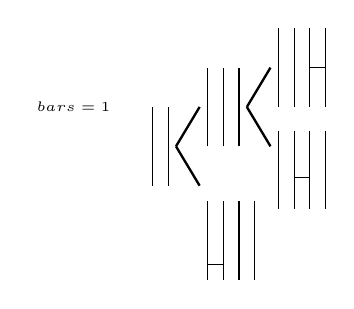
\begin{tikzpicture}
        \node at (-1, 1){\tiny $bars=1$};
        %%l1
          \draw(0, 0) to (0, 1);
          \draw(.2, 0) to (.2, 1);
                      \draw[line width=0.3mm] (.3, .5) to (.6, 1);
                      \draw[line width = .3mm](.3, .5) to (.6, 0);
          %%l2
          \draw(.7, .5) to (.7, 1.5);
          \draw(.9, .5) to (.9, 1.5);
          \draw(1.1, 0.5) to (1.1, 1.5);


            \draw[line width = .3mm](1.2, 1) to (1.5, 1.5);
            \draw[line width = .3mm](1.2, 1) to (1.5, 0.5);
          %%t3 terminate
          \draw(1.6, 1) to (1.6, 2);
          \draw(1.8, 1) to (1.8, 2);
          \draw(2, 1) to (2, 2);
            \draw(2, 1.5) to (2.2, 1.5);
          \draw(2.2, 1) to (2.2, 2);

          %l4 terminate
          \draw(.7, -0.2) to (.7, -1.2);
            \draw(.7, -1) to (.9,-1);
          \draw(.9, -.2) to (.9, -1.2);
          \draw(1.1, -.2) to (1.1, -1.2);
          \draw(1.3, -0.2) to (1.3, -1.2);

          %l5 terminate
          \draw(1.6, .7) to (1.6, -.3);
          \draw(1.8, .7) to (1.8, -.3);
            \draw(1.8, .1) to (2, .1);
          \draw(2, .7) to (2, -.3);
          \draw(2.2, .7) to (2.2, -.3);
        
      \end{tikzpicture}
      

               
    \end{minipage}\\~\\

   %%t3
  \begin{minipage}{.8\textwidth}
     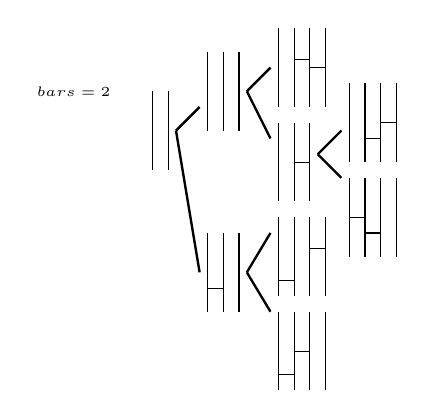
\begin{tikzpicture}
       \node at (-1, 1){\tiny $bars=2$};

        %%L1
        \draw(0, 0) to (0, 1);
        \draw(.2, 0) to (.2, 1);
        
          \draw[line width=.3mm] (.3, .5) to (.6, .8);
          \draw[line width = .3mm](.3, .5) to (.6, -1.3);

        
        \draw(.7, -.8) to (.7, -1.8);
          \draw(.7, -1.5) to (.9, -1.5);
        \draw(.9, -.8) to (.9, -1.8);
        \draw(1.1, -.8) to (1.1, -1.8);

          \draw[line width = .3mm](1.2, -1.3) to (1.5, -.8);
          \draw[line width = .3mm](1.2, -1.3) to (1.5, -1.8);
        
        %%terminate
        \draw(1.6, -.6) to (1.6, -1.6); 
          \draw(1.6, -1.4) to (1.8, -1.4);
         \draw(1.8, -.6) to (1.8, -1.6);  
         \draw(2, -.6) to (2, -1.6);  
            \draw(2, -1) to (2.2, -1); 
         \draw(2.2, -.6) to (2.2, -1.6);
         
         %%terminate
         \draw(1.6, -1.8) to (1.6, -2.8);
          \draw(1.6, -2.6) to (1.8, -2.6);
         \draw(1.8, -1.8) to (1.8, -2.8);
          \draw(1.8, -2.3) to (2, -2.3);
         \draw(2, -1.8) to (2, -2.8);
         \draw(2.2, -1.8) to (2.2, -2.8);



        %%L2 
        \draw(.7, .5) to (.7, 1.5);
        \draw(.9, .5) to (.9, 1.5);
        \draw(1.1, .5) to (1.1, 1.5);

          \draw[line width = .3mm](1.2, 1) to (1.5, 1.3);
          \draw[line width = .3mm](1.2, 1) to (1.5, .4);
        
        %%L3 terminate
        \draw(1.6, .8) to (1.6, 1.8);
        \draw(1.8, .8) to (1.8, 1.8);
          \draw(1.8, 1.4) to (2, 1.4);
        \draw(2, .8) to (2, 1.8);
          \draw(2, 1.3) to (2.2, 1.3);
        \draw(2.2, .8) to (2.2, 1.8);

        %L4 
        \draw(1.6, .6) to (1.6, -.4);
        \draw(1.8, .6) to (1.8, -.4);
          \draw(1.8, .1) to (2, .1);
        \draw(2, .6) to (2, -.4);
          \draw[line width = .3mm](2.1, .2) to (2.4, .5);
          \draw[line width = .3mm](2.1, .2) to (2.4, -.1);
        
        %L5 terminate
        \draw(2.5, .1) to (2.5, 1.1);
        \draw(2.7, .1) to (2.7, 1.1);
          \draw(2.7, .4) to (2.9, .4);
        \draw(2.9, .1) to (2.9, 1.1);
          \draw(2.9, .6) to (3.1, .6);
        \draw(3.1,.1) to (3.1, 1.1);

        %L6 terminate
        \draw(2.5, -.1) to (2.5, -1.1);
          \draw(2.5, -.6) to (2.7, -.6);
        \draw(2.7, -.1) to (2.7, -1.1);
          \draw(2.7, -.8) to (2.9, -.8);
        \draw(2.9, -.1) to (2.9, -1.1);
        \draw(3.1, -.1) to (3.1, -1.1);


      \end{tikzpicture}\hspace{10mm}
      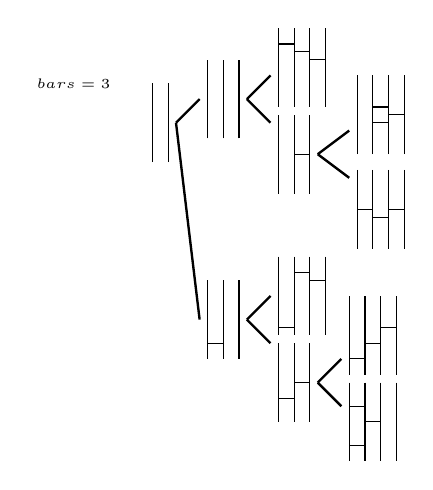
\begin{tikzpicture}
      \node at (-1, 1){\tiny $bars=3$};

        %%L1
           \draw(0, 0) to (0, 1);
           \draw(.2, 0) to (.2, 1);
          
        %%lines 
        \draw[line width = .3mm](.3, .5) to (.6, .8);
        \draw[line width = .3mm](.3, .5) to (.6, -2);
         %% add second line
         
          %L2 
          \draw(.7, .3) to (.7, 1.3);
          \draw(.9, .3) to (.9, 1.3);
          \draw(1.1, .3) to (1.1, 1.3);

        \draw[line width = .3mm](1.2, .8) to (1.5, 1.1);
        \draw[line width = .3mm](1.2, .8) to (1.5, .5);

        %%L3 terminate
        \draw(1.6, .7) to (1.6, 1.7);
          \draw(1.6, 1.5) to (1.8, 1.5);
        \draw(1.8, .7) to (1.8, 1.7);
          \draw(1.8, 1.4) to (2, 1.4);
        \draw(2, .7) to (2, 1.7);
          \draw(2, 1.3) to (2.2, 1.3);
        \draw(2.2, .7) to (2.2, 1.7);

        %%L4 
        \draw(1.6, -.4) to (1.6, .6);
        \draw(1.8, -.4) to (1.8, .6);
          \draw(1.8, .1) to (2, .1);
        \draw(2, -.4) to (2, .6);

        \draw[line width =.3mm](2.1, .1) to (2.5, .4);
        \draw[line width = .3mm](2.1, .1) to (2.5, -.2);

        %%L5 terminate
        \draw(2.6, .1) to (2.6, 1.1);
        \draw(2.8, .1) to (2.8, 1.1);
          \draw(2.8, .5) to (3, .5);
          \draw(2.8, .7) to (3, .7);
        \draw(3, .1) to (3, 1.1);
          \draw(3, .6) to (3.2, .6);
        \draw(3.2, .1) to (3.2, 1.1);

        %%L6 terminate
        \draw(2.6, -.1) to (2.6, -1.1);
          \draw(2.6, -.6) to (2.8, -.6);
        \draw(2.8, -.1) to (2.8, -1.1);
          \draw(2.8, -.7) to (3, -.7);
        \draw(3, -.1) to (3, -1.1);
          \draw(3, -.6) to (3.2, -.6);
        \draw(3.2, -.1) to (3.2, -1.1);

        %%L7 
        \draw(.7, -1.5) to (.7, -2.5);
          \draw(.7, -2.3) to (.9, -2.3);
        \draw(.9, -1.5) to (.9, -2.5);
        \draw(1.1, -1.5) to (1.1, -2.5);
          
          \draw[line width = .3mm](1.2, -2) to (1.5, -1.7);
          \draw[line width = .3mm](1.2, -2) to (1.5, -2.3);
        
      %%L8 terminate
      \draw(1.6, -1.2) to (1.6, -2.2);
        \draw(1.6, -2.1) to (1.8, -2.1);
      \draw(1.8, -1.2) to (1.8, -2.2);
        \draw(1.8, -1.4) to (2, -1.4);
      \draw(2, -1.2) to (2, -2.2);
        \draw(2, -1.5) to (2.2, -1.5);
      \draw(2.2, -1.2) to (2.2, -2.2);
    
      %%L9 
      \draw(1.6, -2.3) to (1.6, -3.3);
        \draw(1.6, -3) to (1.8, -3);
      \draw(1.8, -2.3) to (1.8, -3.3);
        \draw(1.8, -2.8) to (2, -2.8);
      \draw(2, -2.3) to (2, -3.3);

      \draw[line width = .3mm](2.1, -2.8) to (2.4, -2.5);
      \draw[line width = .3mm](2.1, -2.8) to (2.4, -3.1);

      %%L10 terminate
      \draw(2.5, -2.7) to (2.5, -1.7);
        \draw(2.5, -2.5) to (2.7, -2.5);
      \draw(2.7, -2.7) to (2.7, -1.7);
        \draw(2.7, -2.3) to (2.9, -2.3);
      \draw(2.9, -2.7) to (2.9, -1.7);
        \draw(2.9, -2.1) to (3.1, -2.1);
      \draw(3.1, -2.7) to (3.1, -1.7);

      %%L11 terminate
      \draw(2.5, -2.8) to (2.5, -3.8);
        \draw(2.5, -3.6) to (2.7, -3.6);
        \draw(2.5, -3.1) to (2.7, -3.1);
      \draw(2.7, -2.8) to (2.7, -3.8);
        \draw(2.7, -3.3) to (2.9, -3.3);
      \draw(2.9, -2.8) to (2.9, -3.8);
      \draw(3.1, -2.8) to (3.1, -3.8);
    
    \end{tikzpicture}
      
   \end{minipage}\\~\\
  \begin{minipage}{.8\textwidth}
     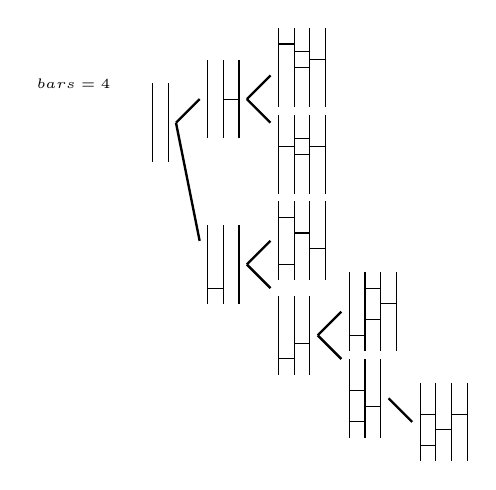
\begin{tikzpicture}
       \node at (-1, 1){\tiny $bars=4$};

      %%L1
      \draw(0, 0) to (0, 1);
      \draw(.2, 0) to (.2, 1);
        \draw[line width = .3mm](.3, .5) to (.6, .8);
        \draw[line width = .3mm](.3, .5) to (.6, -1);
      
        %L2 
          \draw(.7, .3) to (.7, 1.3);
          \draw(.9, .3) to (.9, 1.3);
            \draw(.9, .8) to (1.1, .8);
          \draw(1.1, .3) to (1.1, 1.3);
      
        \draw[line width = .3mm](1.2, .8) to (1.5, 1.1);
        \draw[line width = .3mm](1.2, .8) to (1.5, .5);

        %%L3 terminate
        %%L3 terminate
        \draw(1.6, .7) to (1.6, 1.7);
          \draw(1.6, 1.5) to (1.8, 1.5);
        \draw(1.8, .7) to (1.8, 1.7);
          \draw(1.8, 1.4) to (2, 1.4);
          \draw(1.8, 1.2) to (2, 1.2);
        \draw(2, .7) to (2, 1.7);
          \draw(2, 1.3) to (2.2, 1.3);
        \draw(2.2, .7) to (2.2, 1.7);
        %%L4 termiante
        \draw(1.6, -.4) to (1.6, .6);
          \draw(1.6, .2) to (1.8, .2);
        \draw(1.8, -.4) to (1.8, .6);
          \draw(1.8, .1) to (2, .1);
          \draw(1.8, .3) to (2, .3);
        \draw(2, -.4) to (2, .6);
          \draw(2, .2) to (2.2, .2);
        \draw(2.2, -.4) to (2.2, .6);

        %%L5
        \draw(.7, -.8) to (.7, -1.8);
          \draw(.7, -1.6) to (.9, -1.6);
        \draw(.9, -.8) to (.9, -1.8);
        \draw(1.1, -.8) to (1.1, -1.8);

        \draw[line width=.3mm](1.2, -1.3) to (1.5, -1);
        \draw[line width = .3mm](1.2, -1.3) to (1.5, -1.6);

        %%L6 terminate
        \draw(1.6, -.5) to (1.6, -1.5);
          \draw(1.6, -1.3) to (1.8, -1.3);
          \draw(1.6, -.7) to (1.8, -.7);
        \draw(1.8, -.5) to (1.8, -1.5);
          \draw(1.8, -.9) to (2, -.9);
        \draw(2, -.5) to (2, -1.5);
          \draw(2, -1.1) to (2.2, -1.1);
        \draw(2.2, -.5) to (2.2, -1.5);

        %%L7
        \draw(1.6, -1.7) to (1.6, -2.7);
          \draw(1.6, -2.5) to (1.8, -2.5);
        \draw(1.8, -1.7) to (1.8, -2.7);
          \draw(1.8, -2.3) to (2, -2.3);
        \draw(2, -1.7) to (2, -2.7);

        \draw[line width = .3mm](2.1, -2.2) to (2.4, -1.9);
        \draw[line width = .3mm](2.1, -2.2) to (2.4, -2.5);

        %%L8 terminate
        \draw(2.5, -1.4) to (2.5, -2.4);
          \draw(2.5, -2.2) to (2.7, -2.2);
        \draw(2.7, -1.4) to (2.7, -2.4);
          \draw(2.7, -2) to (2.9, -2);
          \draw(2.7, -1.6) to (2.9, -1.6);
        \draw(2.9, -1.4) to (2.9, -2.4);
          \draw(2.9, -1.8) to (3.1, -1.8);
        \draw(3.1, -1.4) to (3.1, -2.4);

        %%L9
        \draw(2.5, -2.5) to (2.5, -3.5);
          \draw(2.5, -3.3) to (2.7, -3.3);
          \draw(2.5, -2.9) to (2.7, -2.9);
        \draw(2.7, -2.5) to (2.7, -3.5);
          \draw(2.7, -3.1) to (2.9, -3.1);
        \draw(2.9, -2.5) to (2.9, -3.5);

        \draw[line width = .3mm](3, -3) to (3.3, -3.3);
        %%L10 terminate
        \draw(3.4, -2.8) to (3.4, -3.8);
          \draw(3.4, -3.6) to (3.6, -3.6);
          \draw(3.4, -3.2) to (3.6, -3.2);
        \draw(3.6, -2.8) to (3.6, -3.8);
          \draw(3.6, -3.4) to (3.8, -3.4);
        \draw(3.8, -2.8) to (3.8, -3.8);
          \draw(3.8, -3.2) to (4, -3.2);
        \draw(4, -2.8) to (4, -3.8);

    
      \end{tikzpicture}\hspace{10mm}
      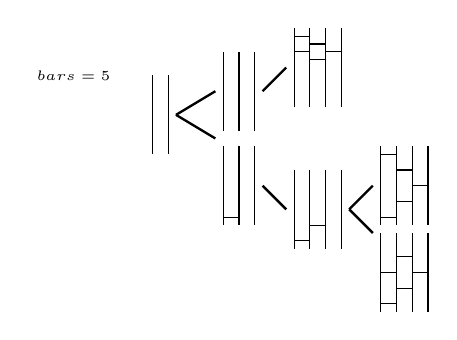
\begin{tikzpicture}
            \node at(-1, 5){\tiny $bars=5$};
       %     %%L1
            \draw(0, 4) to (0, 5);
            \draw(.2, 4) to (0.2, 5);
           
            \draw[line width = .3mm](.3, 4.5) to (0.8, 4.8);
            \draw[line width =.3mm](.3, 4.5) to (.8, 4.2);
 
       %     %%L2
 
            \draw(.9, 4.3) to (.9, 5.3);
            \draw(1.1, 4.3) to (1.1, 5.3);
            \draw(1.3, 4.3) to (1.3, 5.3);
 
            %L3 terminate
            \draw[line width = .3mm](1.4, 4.8) to (1.7, 5.1);
             \draw(1.8, 4.6) to (1.8, 5.6);
               \draw(1.8, 5.3) to (2, 5.3);
              \draw(1.8, 5.5) to (2, 5.5);
             \draw(2, 4.6) to (2, 5.6);
               \draw(2, 5.4) to (2.2, 5.4);
               \draw(2, 5.2) to (2.2, 5.2);
             \draw(2.2, 4.6) to (2.2, 5.6);
               \draw(2.4, 5.3) to (2.2, 5.3);
             \draw(2.4, 4.6) to (2.4, 5.6);
 
      %       %%L4 
             \draw(.9, 4.1) to (.9, 3.1);
               \draw(.9, 3.2) to (1.1, 3.2);
             \draw(1.1, 4.1) to (1.1, 3.1);
             \draw(1.3, 4.1) to (1.3, 3.1);
 
            \draw[line width = .3mm](1.4, 3.6) to (1.7, 3.3);
      %  %      %%L5
             \draw(1.8, 3.8) to (1.8, 2.8);
               \draw(1.8, 2.9) to (2, 2.9);
             \draw(2, 3.8) to (2, 2.8);
               \draw(2, 3.1) to (2.2, 3.1);
             \draw(2.2, 3.8) to (2.2, 2.8);
             \draw(2.4, 3.8) to (2.4, 2.8);
 
            \draw[line width = .3mm](2.5, 3.3) to (2.8, 3);
            \draw[line width = .3mm](2.5, 3.3) to (2.8, 3.6);
       %     %%L6 terminate
            \draw(2.9, 3.1) to (2.9, 4.1);
              \draw(2.9, 3.2) to (3.1, 3.2);
              \draw(2.9, 4) to (3.1, 4);
            \draw(3.1, 3.1) to (3.1, 4.1);
              \draw(3.1, 3.4) to (3.3, 3.4);
              \draw(3.1,3.8) to (3.3, 3.8);
            \draw(3.3, 3.1) to (3.3, 4.1);
              \draw(3.3, 3.6) to (3.5, 3.6);
            \draw(3.5, 3.1) to (3.5, 4.1);
       %     %%L7 terminate
            \draw(2.9, 3) to (2.9, 2);
               \draw(2.9, 2.1) to (3.1, 2.1);
               \draw(2.9, 2.5) to (3.1, 2.5);
            \draw(3.1, 2) to (3.1, 3);
               \draw(3.1, 2.3) to (3.3, 2.3);
               \draw(3.1, 2.7) to (3.3, 2.7);
            \draw(3.3, 2) to (3.3, 3);
               \draw(3.3, 2.5) to (3.5, 2.5);
            \draw(3.5, 2) to (3.5, 3);
        \end{tikzpicture}
   \end{minipage}\\~\\
   \begin{minipage}{.8\textwidth}
    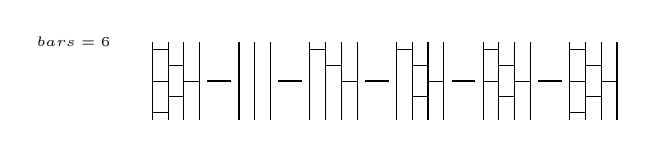
\begin{tikzpicture}
      \draw node at (-1, 1){\tiny $bars=6$};
      \draw(0, 0) to (0, 1);
        \draw(0, .1) to (.2, .1);
        \draw(0, .5) to (.2, .5);
        \draw(0, .9) to (.2, .9);
      \draw(.2, 0) to (.2, 1);
        \draw(.2, .3) to (.4, .3);
        \draw(.2, .7) to (.4, .7);
      \draw(.4, 0) to (.4, 1);
        \draw(.4, .5) to (.6, .5);
      \draw(.6, 0) to (.6, 1);

      \draw[line width = .3mm](.7, .5) to (1, .5);
      %%L2
      \draw(1.1, 0) to (1.1, 1);
      \draw(1.3, 0) to (1.3, 1);
      \draw(1.5, 0) to (1.5, 1);

      \draw[line width = .3mm](1.6, .5) to (1.9, .5);

      %%L3
      \draw(2, 0) to (2, 1);
        \draw(2, .9) to (2.2, .9);
      \draw(2.2, 0) to (2.2, 1);
        \draw(2.2, .7) to (2.4, .7);
      \draw(2.4, 0) to (2.4, 1);
        \draw(2.4, .5) to (2.6, .5);
      \draw(2.6, 0) to (2.6, 1);
    
      \draw[line width=.3mm](2.7, .5) to (3, .5);

      %L4
      \draw(3.1, 0) to (3.1, 1);
        \draw(3.1, .9) to (3.3, .9);
      \draw(3.3, 0) to (3.3, 1);
        \draw(3.3, .7) to (3.5, .7);
        \draw(3.3, .3) to (3.5, .3);
      \draw(3.5, 0) to (3.5, 1);
        \draw(3.5, .5) to (3.7, .5);
      \draw(3.7, 0) to (3.7, 1);

      \draw[line width = .3mm](3.8, .5) to (4.1, .5);

      %L5
      \draw(4.2, 0) to (4.2, 1);
        \draw(4.2, .9) to (4.4, .9);
        \draw(4.2, .5) to (4.4, .5);
      \draw(4.4, 0) to (4.4, 1);
        \draw(4.4, .7) to (4.6, .7);
        \draw(4.4, .3) to (4.6, .3);
      \draw(4.6, 0) to (4.6, 1);
        \draw(4.6, .5) to (4.8, .5);
      \draw(4.8, 0) to (4.8, 1);
    
      %%L6 terminate
      \draw[line width = .3mm](4.9, .5) to (5.2, .5);
      \draw(5.3, 0)  to (5.3, 1);
        \draw(5.3, .9) to (5.5, .9);
        \draw(5.3, .5) to (5.5, .5);
        \draw(5.3, .1) to (5.5, .1);
      \draw(5.5, 0)  to (5.5, 1);
        \draw(5.5, .7) to (5.7, .7);
        \draw(5.5, .3) to (5.7, .3);
      \draw(5.7, 0)  to (5.7, 1);
        \draw(5.7, .5) to (5.9, .5);
      \draw(5.9, 0)  to (5.9, 1);
    \end{tikzpicture}
    
   \end{minipage}
  \caption{The forest for all ladders in $CanL\{\pi_{4}\}$ generated by the Cyclic Inversion Algorithm. The first tree has all ladders with zero bars, the second tree 
  has all ladders with 1 bar, etc. }
\end{figure}\pagebreak

It has been stated that the forest created by the Cyclic Inversion algorithm generates $CanL\{\pi_{N}\}$. This claim has 
yet to have been proven, so the following lemma will prove this claim.

\begin{lemma}
  The forest created by the Cyclic Inversion algorithm generates $CanL\{\pi_{N}\}$
\end{lemma}
\begin{proof}
  The proof is done by way of contradiction. Suppose that the cyclic inversion algorithm generated $N!$ ladders and did not generate $CanL\{\pi_{N}\}$, 
  then there would be two or more ladders generated by the cyclic inversion algorithm which belonged to the same $OptL\{\pi_{N}\}$. If that were the 
  case, then at least one of these ladders would not be the root ladder from the $OptL\{\pi_{N}\}$. However, it was already stated that the canonical 
  representative for $CanL\{\pi_{N}\}$ was the root ladder from each $OptL\{\pi_{N}\}$, which leads to a contradiction. Therefore each ladder generated 
  by the cyclic inversion algorithm is part of $CanL\{\pi_{N}\}$. 
\end{proof}

For each tree in the forest, the algorithm effectively relocates one or more bars from the $Kth$ route to the the $K-1th$ route 
until the $K-1th$ route has either no more space left for bars, i.e. the $K-1th$ route has $K-2$ bars in the ladder or the number of 
bars in the ladder is equal to the current limit. This is what is happening when 
a bar is added to some route; it only gets added once the bar of a greater route has been removed unless the route is $K=N$. When $K=N$, 
bars are continuously added to the $K=Nth$ route until no more bars can be added for $K=N$ or the number of bars is equal to the current limit. 
For example, suppose $N=5$ and the current limit for the number of bars is three, then when $K=N$, the first ladder for this forest will 
be the ladder in which all three bars belong to the fifth route. Seeing as element $5$ has at most four bars in the ladder. However, 
if the current limit is 6, then the first ladder in the forest will have all the bars belonging to the fifth root as well as the first two bars 
belonging to the fourth root, seeing as the $5th$ element has at most $4$ bars, yet the given current limit for the number of bars is six. Once 
all the bars for the $K=Nth$ route have been added, the upper leftmost bar of the $K=Nth$ route is relocated to the $N-1th$ route, this process 
continues until the $N-1th$ route has had all of its bars added. Upon completion, all the bars are removed from the $N-1th$ route, and the 
first bar of the $N-2th$ route is added. Then the algorithm repeats itself by adding all the bars to the $K=Nth$ route until the current limit 
is reached or the $Nth$ route has $N-1$ bars added to the ladder. Again, the upper left most bar 
of the $K=Nth$ route is relocated to the $N-1th$ route; this continues until the number of bars added is equal to the current limit or 
the $N-1th$ route has $N-2$ bars added, keeping in mind that the $N-2th$ route now has a bar in the ladder. Once complete, all the bars of the 
$N-1th$ route are removed, and the next bar of the $N-2th$ route is added if possible or all the bars of the $N-2th$ route are removed, and the 
first bar of the $N-3rd$ route is added. The forest terminates when the number of bars in the ladder is equal to the current limit and 
each bar in the ladder belongs to the smallest route(s). For example, if $N=4$ and the current limit for the number of bars is three, then 
the ladder which terminates the forest for $CurrentLimit=3$ is the ladder with one bar belonging to route $2$ and two bars belonging to route 
$3$. It must be noted that the row and column calculation for the insertion of a bar is the same as the SJT algorithm which is why the proofs 
for the row and column calculation are not provided for the Cyclic Inversion algorithm. 
